\chapter{Fusione tramite deep learning}

\section{Le componenti della CNN}
\subsection{Reti neurali residuali}
Le reti neurali residuali, o ResNet, sono stati introdotti da Microsoft nel 2015 battendo il record della competizione ILSVRC con un errore del 3.6\%, superando per la prima volta le prestazioni umane.\\
L'idea che sta alla base delle reti neurali residuali è l'utilizzo di un particolare tipo di blocco, il \textit{residual block}, che sfrutta il concetto delle \textit{skip connection}. \\
Vediamo ora il modello del residual block:
\begin{figure}[ht]
    \centering
    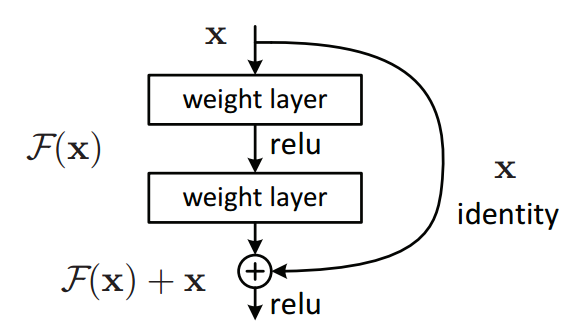
\includegraphics[width=0.5\columnwidth]{res_block.png}
    \caption[Residual block]{Schema del residual block}
\end{figure}\\
Ogni blocco consiste in una serie di strati, ottenendo una certa $F(x)$, seguito da una \textit{skip connection} che aggiunge al risultato l'input del blocco stesso. Dunque in uscita dal blocco si ha
$$ H(x)=F(x)+x $$
Attraverso la concatenazione di blocchi di questo tipo, ResNet impara a predire l'output non attraverso l'apprendimento di una trasformazione diretta dei dati di input, ma attraverso l'apprendimento del termine $F(x)$, detto \textit{residuo}, da sommare al dato di input per arrivare all'output. Tale modello semplifica la costruzione di strati di identità, basta infatti spingere $F(x)$ verso zero e lasciare l'output come x. Ciò permette agli strati più profondi della rete di alterare poco i concetti già appresi dagli strati precedenti, preservando così le informazioni. Questa architettura ha permesso di creare reti molto più profonde, fino a 152 strati.

\subsection{Batch Normalization}
Durante il processo di addestramento, gli esempi del training set vengono processati in gruppi, detti mini-batch, di dimensione fissa per velocizzare la fase di train sfruttando il parallelismo offerto dalle GPU. La \textit{Batch Normalization} è una tecnica che consiste nel normalizzare i dati del mini-batch ad ogni strato intermedio della rete. In questo modo si riduce il così detto \textit{Internal Covariance Shift}. L'utilizzo del batch normalization ha l'intento di velocizzare il training della rete neurale e migliorarne la stabilità e le performance. Questa operazione si è rivelata particolarmente efficace nelle reti neurali residuali.

\subsection{Convoluzione dilatata}
\subsection{Convoluzioni 1x1}

\section{la rete neurale selezionata}

\section{Il processo di training}
\subsection{Loss function e ottimizzazione}
\subsection{Inizializzazione delle variabili}
\subsection{Iperparametri}
batch size e learning rate
\subsection{Early stopping}